\section{Ход работы}

В таблице представлены данные о продаже шариковых ручек изготовителя \textit{Click}, а также данные для анализа эффективности маркетинговых усилий в фирме -- реклама и торговые представители. Необходимо произвести регрессионный анализ данных.

Изначально были построены парные регрессии показателя продаж на каждый из факторов. Также были построены диаграммы исходных данных с линией регрессии, остатков на фактор и остатков на номера наблюдений. Были исследованы статистические значимости коэффициентов для каждой из регрессий.

\begin{figure}[H]
	\begin{minipage}[H]{0.32\linewidth}
		\begin{center}
			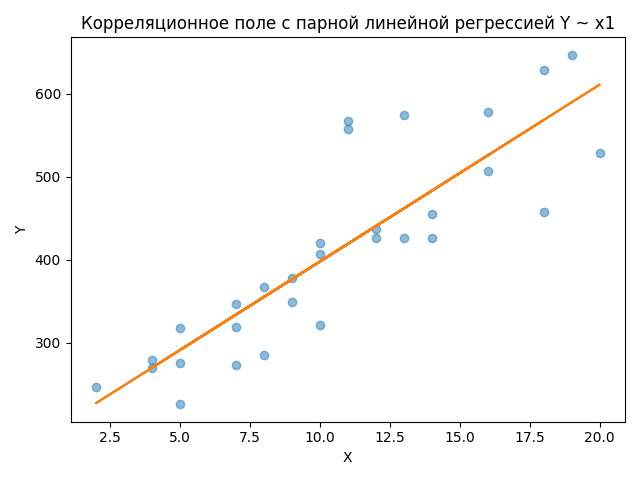
\includegraphics[width=\linewidth]{figures/lin_reg_y_x1}
		\end{center}
	\end{minipage}
	\hfill
	\begin{minipage}[H]{0.32\linewidth}
		\begin{center}
			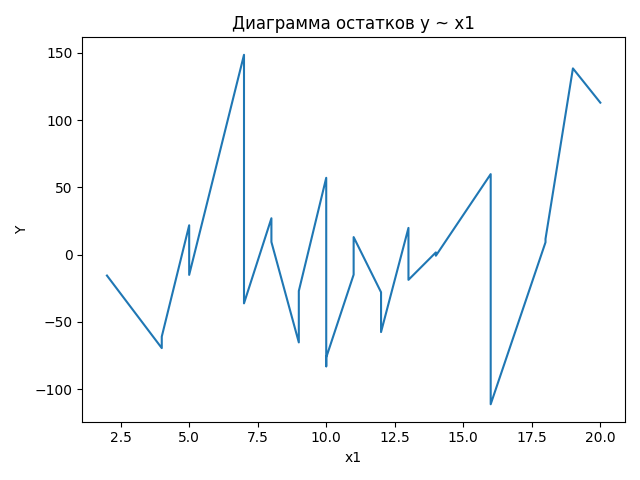
\includegraphics[width=\linewidth]{figures/res_plot_x1}
		\end{center}
	\end{minipage}
	\hfill
	\begin{minipage}[H]{0.32\linewidth}
		\begin{center}
			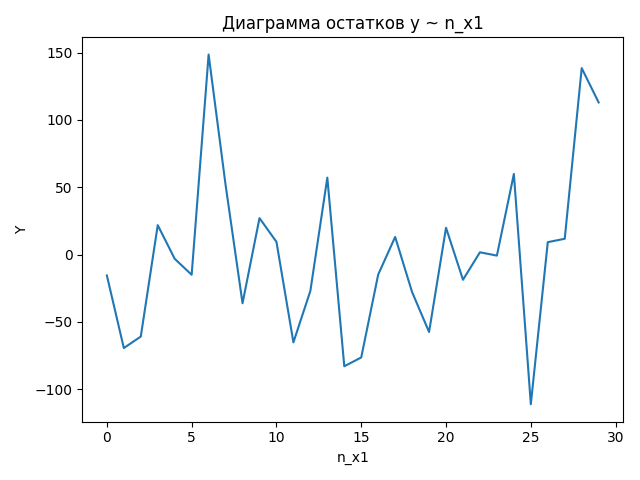
\includegraphics[width=\linewidth]{figures/res_plot_n_x1}
		\end{center}
	\end{minipage}
\end{figure}

\begin{figure}[H]
	\begin{minipage}[H]{0.32\linewidth}
		\begin{center}
			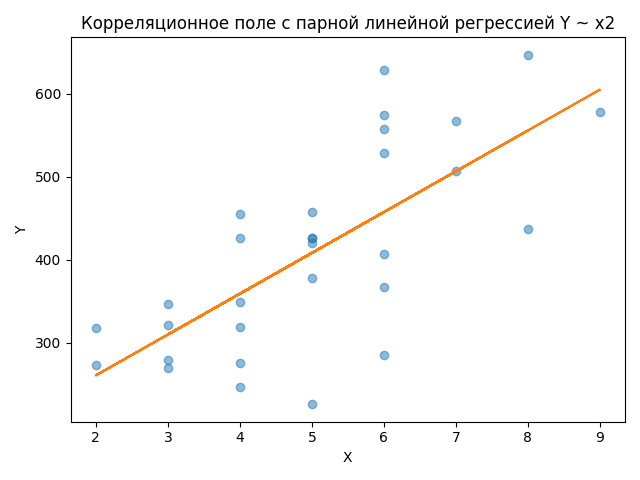
\includegraphics[width=\linewidth]{figures/lin_reg_y_x2}
		\end{center}
	\end{minipage}
	\hfill
	\begin{minipage}[H]{0.32\linewidth}
		\begin{center}
			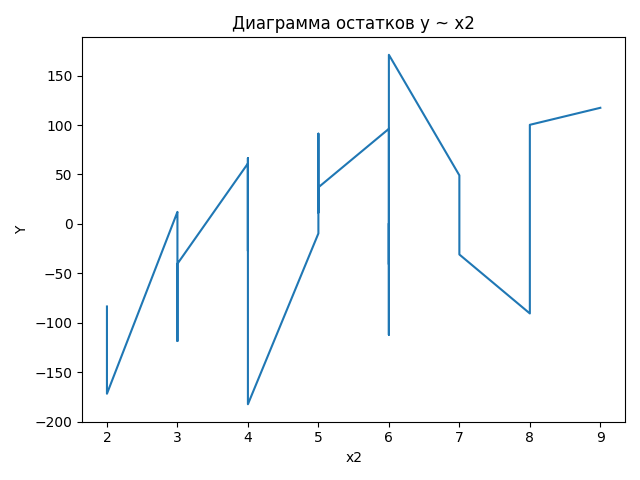
\includegraphics[width=\linewidth]{figures/res_plot_x2}
		\end{center}
	\end{minipage}
	\hfill
	\begin{minipage}[H]{0.32\linewidth}
		\begin{center}
			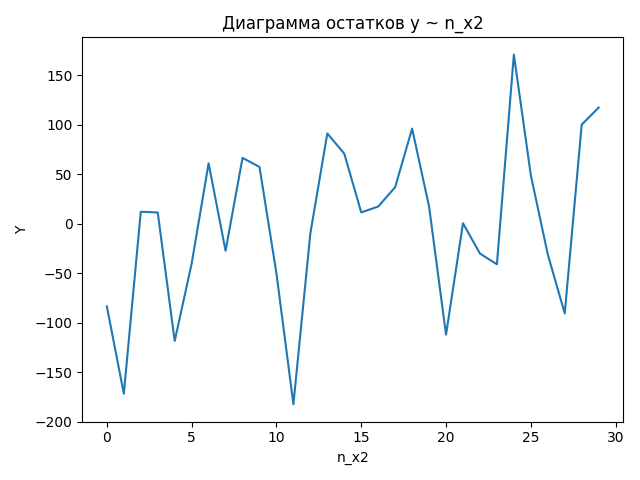
\includegraphics[width=\linewidth]{figures/res_plot_n_x2}
		\end{center}
	\end{minipage}
\end{figure}

В соответствии с заданием, была построена множественная регрессия, где также построены диаграмма остатков на номера наблюдений и прогноз показателя продаж.

\begin{figure}[H]
	\begin{center}
		\begin{minipage}[H]{0.7\linewidth}
				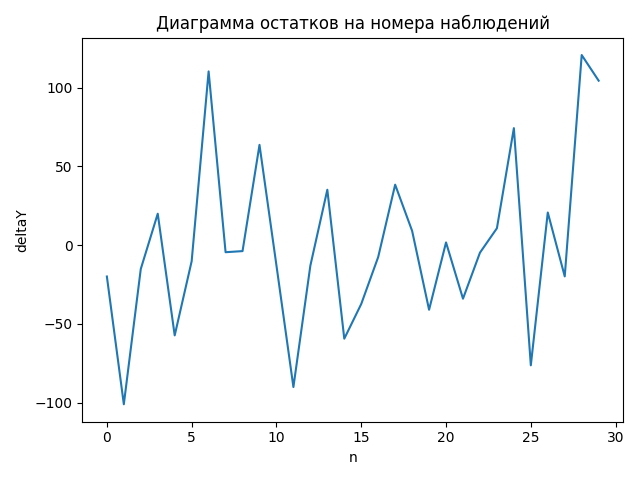
\includegraphics[width=\linewidth]{figures/res_plot_gen}
		\end{minipage}
	\end{center}
\end{figure}

Все результаты представлены как вывод в консоль Python вышеописанных значений. Исходя из результатов и построенных графиков, можно сделать вывод, что оба фактора существенно значимы для продаж. Второй фактор имеет больший угловой коэффициент (если сравнивать парные регрессии), а, значит, вносит больший вклад в получение дохода от продаж. Прогнозирование множественной регрессии имеет и значение, и интервал больше, чем в парных, что ещё раз доказывает существенную значимость обоих факторов.

\VerbatimInput{figures/file.txt}
\VerbatimInput{figures/data.txt}